% Pitchbook-style summary of the hypothetical cat bond. Built by scripts/make_pitchbook.py,
% which writes every number (build/numbers.tex), table (build/tab_*.tex) and figure
% (build/fig_*.pdf) from the files in results/. This file contains no numbers of its own.
\documentclass[12pt]{article}
\usepackage[letterpaper,landscape,margin=0.7in,footskip=0.35in]{geometry}
\usepackage[T1]{fontenc}
\usepackage[scaled]{helvet}
\renewcommand{\familydefault}{\sfdefault}
\usepackage{graphicx,booktabs,tabularx,xcolor,fancyhdr,lastpage,enumitem,tikz}
\usetikzlibrary{arrows.meta,positioning}
\definecolor{accent}{HTML}{2A78D6}
\definecolor{ink}{HTML}{0B0B0B}
\definecolor{muted}{HTML}{52514E}
\definecolor{warn}{HTML}{C00000}
\input{build/numbers.tex}
\pagestyle{fancy}
\fancyhf{}
\renewcommand{\headrulewidth}{0pt}
\fancyfoot[L]{\small\color{warn}\textbf{Illustrative, hypothetical sponsor, not an offering}}
\fancyfoot[R]{\small\color{muted}Teaching-grade model \quad Page \thepage\ of \pageref{LastPage}}
\setlist{nosep,leftmargin=1.2em}
\setlength{\parindent}{0pt}
\setlength{\parskip}{4pt}
\newcommand{\slide}[1]{\newpage{\color{accent}\Large\textbf{#1}}\par\vspace{2pt}{\color{accent}\rule{\linewidth}{1pt}}\par\vspace{4pt}}
\begin{document}
\thispagestyle{fancy}
\vspace*{0.6in}
{\color{accent}\Huge\textbf{Florida Named-Storm Catastrophe Bond}}\par\vspace{8pt}
{\LARGE Three-layer per-occurrence structure for a hypothetical homeowners insurer}\par\vspace{18pt}
{\large Teaching-grade illustration: simulated hurricane event set fitted to HURDAT2 (1900--2019),
hypothetical USD \numTIVbn{} billion portfolio, spread range from a regression on
\numNLayers{} public tranche prices.}\par\vspace{30pt}
\fcolorbox{warn}{white}{\parbox{0.9\linewidth}{\large\color{warn}\textbf{Illustrative only.}
\color{ink} The sponsor and its portfolio are hypothetical. This document is not an offering of
securities, a quote, a recommendation or investment advice. The loss model is a teaching-grade
model built from public data, not a vendor catastrophe model (RMS, Verisk, CoreLogic); its
expected losses are not comparable to those in a cat bond offering circular. CLIMADA was not
used. Spread figures are regression outputs, not prices.}}
\par\vfill
{\color{muted}Generated from the results files of the cat-bond-issuance-model repository
(scripts/make\_pitchbook.py). Every number in this document is read from a file in
\texttt{results/}.}

\slide{Transaction summary (hypothetical)}
Three adjacent per-occurrence layers of USD \numLayerLimitUSDm{} million each
(USD \numTotalLimitUSDm{} million in total) on a hypothetical Florida homeowners portfolio,
chosen by a rule fixed before any spread was fitted: the stack of grid layers whose expected
losses are closest to 4\%, 2\% and 1\% of limit.\par\vspace{6pt}
\centering
\input{build/tab_summary.tex}\par\vspace{6pt}
\raggedright\normalsize
\begin{itemize}
\item AP: probability that at least one event in a year reaches the attachment. EP: probability
  that the whole layer is lost within a year. EL: mean annual principal loss over the limit
  (annual loss capped at the limit). All annual, from 100,000 simulated years (seed 1).
\item EL band: 5\% and 95\% quantiles over \numNBand{} refits of the hazard model on bootstrap
  samples of the 1900--2019 years (frequency, intensity and landfall pool only, not model form).
\item Spreads: median and 90\% prediction interval from M1 (log spread on log EL) and M2 (plus
  issue-year effects, 2025) fitted on public layers. A regression output, not a quote.
\item Probability of any principal loss over a 3-year term: \numPThreeBot\%, \numPThreeMid\% and
  \numPThreeTop\% (bottom, middle, top).
\end{itemize}

\slide{Structure}
\centering
\resizebox{\linewidth}{!}{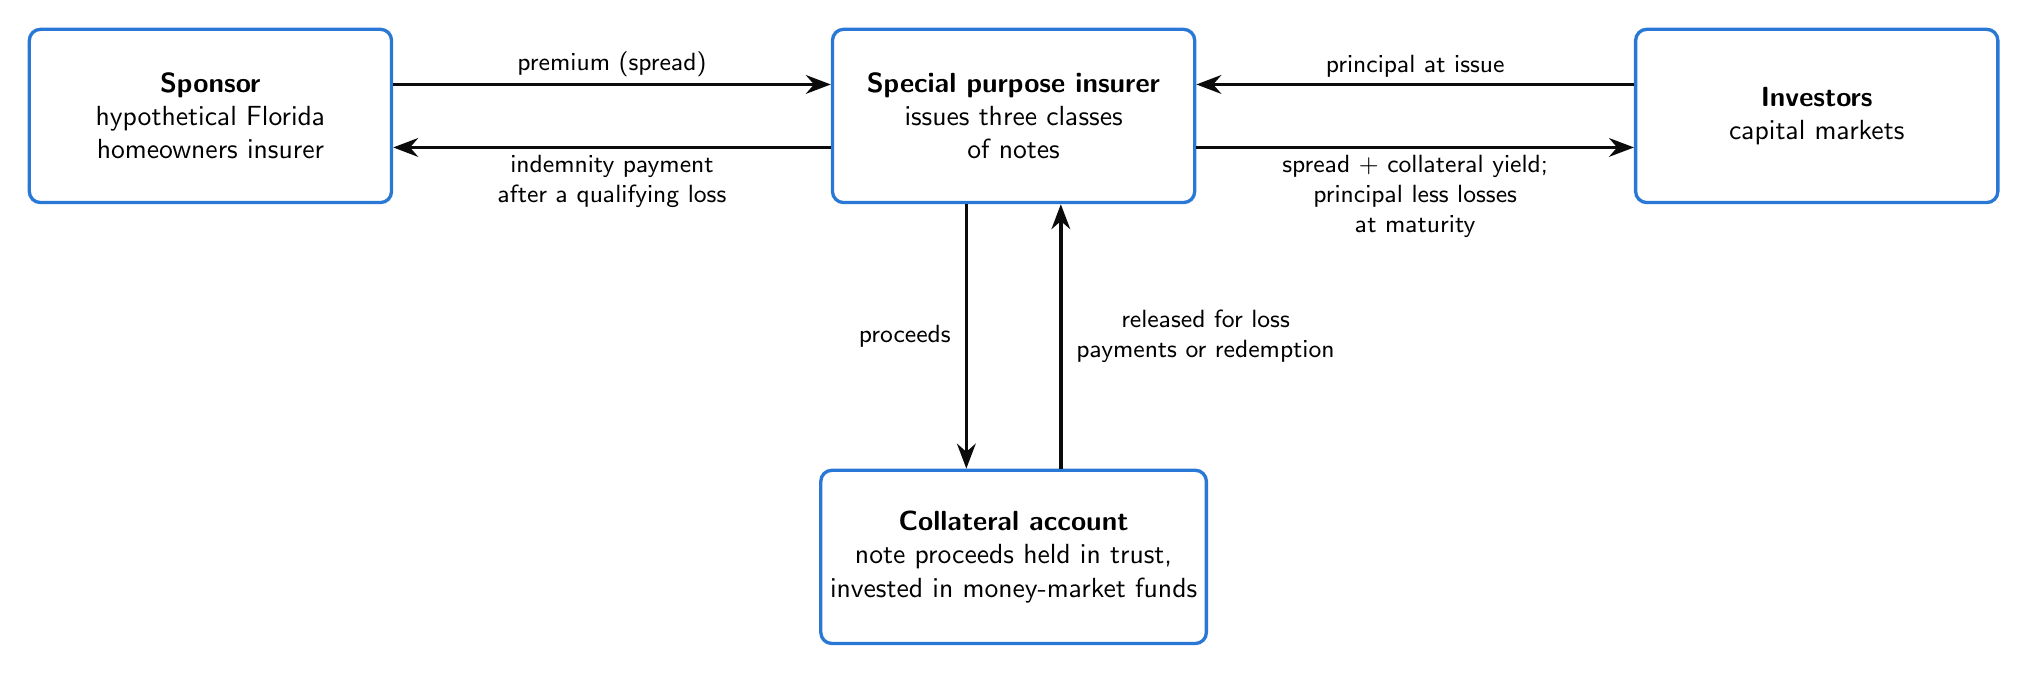
\begin{tikzpicture}[
  box/.style={draw=accent,line width=1.2pt,rounded corners=4pt,minimum width=4.6cm,
    minimum height=2.2cm,align=center,font=\normalsize,fill=white},
  arr/.style={-{Stealth[length=9pt]},line width=1.3pt,draw=ink},
  lab/.style={font=\small,align=center,inner sep=2pt}]
\node[box] (sp) at (0,0) {\textbf{Sponsor}\\hypothetical Florida\\homeowners insurer};
\node[box] (spi) at (10.2,0) {\textbf{Special purpose insurer}\\issues three classes\\of notes};
\node[box] (inv) at (20.4,0) {\textbf{Investors}\\capital markets};
\node[box] (col) at (10.2,-5.6) {\textbf{Collateral account}\\note proceeds held in trust,\\invested in money-market funds};
\draw[arr] ([yshift=4mm]sp.east) -- node[lab,above]{premium (spread)} ([yshift=4mm]spi.west);
\draw[arr] ([yshift=-4mm]spi.west) -- node[lab,below]{indemnity payment\\after a qualifying loss} ([yshift=-4mm]sp.east);
\draw[arr] ([yshift=4mm]inv.west) -- node[lab,above]{principal at issue} ([yshift=4mm]spi.east);
\draw[arr] ([yshift=-4mm]spi.east) -- node[lab,below]{spread + collateral yield;\\principal less losses\\at maturity} ([yshift=-4mm]inv.west);
\draw[arr] ([xshift=-6mm]spi.south) -- node[lab,left=3pt]{proceeds} ([xshift=-6mm]col.north);
\draw[arr] ([xshift=6mm]col.north) -- node[lab,right=3pt]{released for loss\\payments or redemption} ([xshift=6mm]spi.south);
\end{tikzpicture}}\par\vspace{12pt}
\raggedright
\begin{itemize}
\item Trigger: indemnity on the sponsor's (hypothetical) portfolio losses, per occurrence; every
  event in a year can erode principal, capped at each layer's limit.
\item Layers attach at \numAttBot\%, \numAttMid\% and \numAttTop\% of total insured value and
  exhaust at \numExhTop\% for the top layer; they sit above the sponsor's retention.
\item The generic structure is shown for teaching; legal terms, reset, extension and collateral
  rules of a real transaction are not modelled.
\end{itemize}

\slide{Exposure summary (hypothetical portfolio)}
\begin{minipage}[t]{0.52\linewidth}\vspace{0pt}
\includegraphics[width=\linewidth]{build/fig_exposure.pdf}
\end{minipage}\hfill
\begin{minipage}[t]{0.44\linewidth}\vspace{0pt}
Total insured value USD \numTIVbn{} billion (hypothetical) spread over the \numNCounties{}
Florida counties in proportion to 2020 Census households (UF BEBR table), placed at county
centroids. The ten largest counties hold \numTopTenShare\% of the value.\par\vspace{6pt}
\small\input{build/tab_exposure.tex}\par\vspace{6pt}
\normalsize No real insurer's book is used. A real portfolio differs by footprint, distance to
the coast, construction and policy terms; deductible 2\% of value, applied to the county mean
damage ratio.
\end{minipage}

\slide{Hazard and loss model; what was checked and what is weak}
\begin{minipage}[t]{0.5\linewidth}\vspace{0pt}
\textbf{Model.}
\begin{itemize}
\item Florida hurricane landfalls 1900--2019 (HURDAT2): \numNLandfalls{} landfalls, mean
  \numFreqMean{} per year (95\% \numFreqLo--\numFreqHi). Poisson kept (negative binomial test
  p = \numNBp); trend p = \numTrendP.
\item Intensity: generalized Pareto on wind above 64 kt (shape \numGPDxi, scale \numGPDsigma{} kt,
  KS distance \numKSgpd).
\item Track: historical landfall position, heading and speed resampled with jitter; Holland
  wind profile; Kaplan--DeMaria inland decay; Emanuel (2011) damage function.
\item Landfall definition (1966--1984): on 6-hourly fixes only, the geometric rule finds
  \numDefSynAgree{} of \numDefN{} flagged landfalls of other years, with winds \numDefSynWind{} kt
  lower on average.
\end{itemize}
\textbf{Weak points.}
\begin{itemize}
\item Fit 1900--1979, predict 1980--2019: \numOOSpred{} hurricanes predicted, \numOOSobs{}
  observed (p = \numOOSp). No category falls outside its interval, but the intervals are wide:
  the check has little power and says nothing about losses.
\item Window 1950--2019 gives \numAltWindowMean{} per year and the \numAltWindowChoice{} model
  (p = \numAltWindowP); the layer ELs fall to \numWindowMid\% for the middle layer (sensitivity page).
\item No surge, rain, terrain or building inventory; straight tracks; losses not calibrated to
  any insured loss.
\end{itemize}
\end{minipage}\hfill
\begin{minipage}[t]{0.46\linewidth}\vspace{0pt}
\textbf{Out-of-sample check by Saffir-Simpson category} (counts 1980--2019)\par\vspace{4pt}
\small\resizebox{\linewidth}{!}{\input{build/tab_oos.tex}}
\end{minipage}

\slide{Loss exceedance curve with hazard-parameter band}
\begin{minipage}[t]{0.6\linewidth}\vspace{0pt}
\includegraphics[width=\linewidth]{build/fig_lec.pdf}
\end{minipage}\hfill
\begin{minipage}[t]{0.37\linewidth}\vspace{0pt}
\small\resizebox{\linewidth}{!}{\input{build/tab_rp.tex}}\par\vspace{8pt}\normalsize
1-in-100 occurrence loss \numOEPhundred\% of TIV (Monte Carlo SE \numOEPhundredSE); across
\numNBand{} hazard refits the 5--95\% range is \numOEPhundredLo--\numOEPhundredHi\%. Average
annual loss \numAAL\% of TIV.\par\vspace{4pt}
The band reflects uncertainty in frequency, intensity and the landfall pool (10,000 years per
refit). Model-form choices move losses much more (sensitivity page). Shaded horizontal bands:
the three layers.
\end{minipage}

\slide{Layer analytics}
\begin{minipage}[t]{0.55\linewidth}\vspace{0pt}
\textbf{Candidate layers with a limit of 0.5\% of TIV} (base case, 100,000 years)\par\vspace{4pt}
\small\resizebox{\linewidth}{!}{\input{build/tab_grid.tex}}
\end{minipage}\hfill
\begin{minipage}[t]{0.41\linewidth}\vspace{0pt}
\begin{itemize}
\item Each row is a per-occurrence layer; EL falls quickly with the attachment, AP faster than
  EP.
\item The chosen layers are the rows attaching at \numAttBot, \numAttMid{} and \numAttTop\% of
  TIV, with EL \numELBot, \numELMid{} and \numELTop\% (Monte Carlo SE \numELseBot, \numELseMid,
  \numELseTop).
\item EP counts total loss of a layer within a year, including by several partial events.
\item The reference layer (\numRefAtt--\numRefExh\% of TIV, the rounded 1-in-50 to 1-in-100
  occurrence losses) has EL \numRefEL\%.
\end{itemize}
\end{minipage}

\slide{Pricing: regression on public tranche prices}
\begin{minipage}[t]{0.52\linewidth}\vspace{0pt}
\includegraphics[width=\linewidth]{build/fig_pricing.pdf}\par
\small \numNLayers{} distinct layers, \numNSeries{} series, \numNSponsors{} sponsors, issued
2017--2025 (Artemis pages). Deal ELs come from each deal's own vendor model.
\end{minipage}\hfill
\begin{minipage}[t]{0.45\linewidth}\vspace{0pt}
\small\resizebox{\linewidth}{!}{\input{build/tab_slope.tex}}\par\vspace{6pt}
\normalsize Pre-specified rule: proportionality (b = 1) is rejected only if the series wild
bootstrap interval (\numNBoot{} draws) excludes 1 in M1 and M2. Main sample:
M1 \numbOne{} [\numbOneLo, \numbOneHi], M2 \numbTwo{} [\numbTwoLo, \numbTwoHi]: rejected, but in
only \numNRejected{} of \numNSamples{} pre-specified samples (next page).
R-squared \numRsqOne{} (M1), \numRsqTwo{} (M2): issue year explains more than EL. Holding out a
series, M2 misses by \numCVseriesPP{} points of spread (RMSE).
\end{minipage}

\slide{Pricing: robustness and comparable deals}
\begin{minipage}[t]{0.5\linewidth}\vspace{0pt}
\textbf{Slope in every pre-specified sample}\par\vspace{4pt}
\footnotesize\resizebox{\linewidth}{!}{\input{build/tab_prop.tex}}\par\vspace{8pt}\normalsize
\textbf{Caveats.} Programs were chosen by name; two sponsors give most layers; median spread/EL
multiple by issue year runs from \numMultMin{} (\numMultMinYear) to \numMultMax{}
(\numMultMaxYear); ELs are offering-stage figures from different vendor models; three prices are
guidance and four are discount-note equivalents. Leave-one-sponsor-out RMSE \numCVsponsorPP{}
points. The model's EL and the deals' ELs are on different scales.
\end{minipage}\hfill
\begin{minipage}[t]{0.47\linewidth}\vspace{0pt}
\textbf{Five nearest public layers by EL and year}\par\vspace{4pt}
\footnotesize\resizebox{\linewidth}{!}{\input{build/tab_comps.tex}}
\end{minipage}

\slide{Sensitivities of layer EL and implied spread}
\begin{minipage}[t]{0.47\linewidth}\vspace{0pt}
\includegraphics[width=\linewidth]{build/fig_sens.pdf}
\end{minipage}\hfill
\begin{minipage}[t]{0.5\linewidth}\vspace{0pt}
\footnotesize\resizebox{\linewidth}{!}{\input{build/tab_sens.tex}}
\end{minipage}\par\vspace{6pt}
Same seed and 100,000 years per variant. The half-damage wind of the damage function moves the
middle-layer EL to \numVhalfMid\% and the 1950--2019 window to \numWindowMid\%; the public deals
span EL \numDealELmin--\numDealELmax\%, so spreads mapped from ELs outside that range are
extrapolations.

\slide{Limitations}
\begin{itemize}[itemsep=4pt]
\item \textbf{Teaching-grade loss model.} County-centroid exposure, a parametric wind field,
  straight tracks, no storm surge, rainfall, terrain, building inventory or demand surge; no
  calibration to insured losses. Model-form choices (damage function, decay, wind radius)
  move layer EL far more than the hazard-parameter band.
\item \textbf{Hypothetical portfolio.} Value spread by households, not insured values; one
  deductible applied to county mean damage.
\item \textbf{Hazard record.} 120 years of landfalls; the 1966--1984 landfall flags are missing
  in the data file and a geometric rule replaces them; intensity is drawn independently of
  location.
\item \textbf{Deal data.} Only Artemis pages, programs chosen by name, offering-stage ELs from
  different vendor models, a few guidance and discount-note prices; transcription re-checked on
  30 rows, not the source itself.
\item \textbf{Pricing regression.} Year effects absorb the market cycle; errors correlated
  within series and sponsor; leave-one-series-out RMSE \numCVseriesPP{} points of spread; mapping this
  model's EL through it assumes a common EL scale that is not shown.
\item \textbf{Not modelled.} Collateral yield, term structure, reset and extension provisions,
  ratings, investor demand, fees and expenses.
\end{itemize}

\slide{Appendix: assumptions and sources}
\small
\begin{tabularx}{\linewidth}{@{}lX@{}}
\toprule
Item & Assumption or source \\
\midrule
Track data & HURDAT2 Atlantic best tracks (NOAA NHC; Landsea and Franklin 2013), GitHub copies pinned by SHA-256 \\
Calibration window & 1900--2019 (pre-specified); 1950--2019 and 1900--2024 as sensitivities \\
Wind field & Holland (1980) profile; radius of maximum wind and B from Willoughby and Rahn (2004) \\
Inland decay & Kaplan and DeMaria (1995), NHC operational constants \\
Damage & Emanuel (2011): threshold 50 kt, half-damage 150 kt (110 kt and 145.2 kt as sensitivities) \\
Exposure & 2020 Census households by county (UF BEBR); TIV hypothetical; 2\% deductible \\
Simulation & 100,000 years, seed 1; hazard-parameter band from 200 year-bootstrap refits \\
Deal terms & Artemis deal directory pages, accessed 2026-11-05; two transcription checks (the first by the collector) \\
Regression & OLS of log spread on log EL; HC3 (MacKinnon and White 1985), cluster-robust
(Cameron and Miller 2015), wild cluster bootstrap (Cameron, Gelbach and Miller 2008; Roodman et al.\ 2019) \\
Protocol & All models, samples and the layer rule fixed in docs/pricing\_protocol.md before the first fit \\
Files & results/transaction/, results/pricing/, results/eventset/, results/param\_uncertainty/ \\
\bottomrule
\end{tabularx}\par\vspace{6pt}
\textbf{References.} Cameron, Gelbach and Miller (2008), Review of Economics and Statistics
90(3); Cameron and Miller (2015), Journal of Human Resources 50(2); Emanuel (2011), Weather,
Climate, and Society 3; Holland (1980), Monthly Weather Review 108(8); Kaplan and DeMaria (1995),
Journal of Applied Meteorology 34; Landsea and Franklin (2013), Monthly Weather Review 141;
MacKinnon and White (1985), Journal of Econometrics 29(3); Roodman, MacKinnon, Nielsen and Webb
(2019), Stata Journal 19(1); Willoughby and Rahn (2004), Monthly Weather Review 132.
\end{document}
